As this thesis work is a partnership with the local public healthcare administration \ausl{},
this chapter focuses on providing context on information systems used in healthcare and the trends in digital transformation that have been shaping the sector in recent years.
These have been driven by \ac{IoT} and \ac{AI} technologies,
enabling the automatic acquisition of large amounts of data, which need to be integrated across different systems and analyzed to extract useful information to support clinical decisions, motivating the need for interoperability and knowledge representation.
%
The chapter provides an overview of the complexity of \ac{HIS},
the main medical standards, and, finally, the context of \ausl{} and its digital transformation journey.

%=======================================================
\section{Healthcare 4.0}
%=======================================================

As any industrial sector, healthcare is constantly innovated by the introduction of new technologies.
%
The adoption of \ac{ICT} technologies has been driving a digital transformation in healthcare~\cite{Kraus_Schiavone_Pluzhnikova_Invernizzi_2021} which has led healthcare institutions to require new digital capabilities to support their operations and manage the amount of clinical data they produce in order to improve quality of care and reduce costs. 

Compared to other application domains, healthcare is particularly critical for a variety of societal factors, 
including the sensitivity of the personal medical data being handled, the need for high reliability and availability of services, and the complexity of the domain itself, which involves a wide range of stakeholders and professionals. 
%
This makes healthcare generally more conservative in adopting new technologies, making the process of digital transformation generally slower than in other sectors~\cite{Hermes_Riasanow_Clemons_Böhm_Krcmar_2020}.
%
It is then not surprising that despite the \emph{Industry 4.0} paradigm introduced in the early 2010s~\cite{Lasi_Fettke_Kemper_Feld_Hoffmann_2014} and progressively adopted in many sectors is still far from being realized in healthcare today~\cite{Kotzias_Bukhsh_Arachchige_Daneva_Abhishta_2022}.

Healthcare 4.0~\cite{Tortorella_Fogliatto_Mac_Cawley_Vergara_Vassolo_Sawhney_2020} is a term that has been used to refer to the application of Industry 4.0 technological drivers in healthcare.
%
These include \ac{IoT}, Big Data and \ac{AI} technologies, which ease the collection and analysis of large amounts of data, support the continuous care and remote monitoring of patients and the support of clinical decisions through data-driven approaches.
%
The general consensus is that Healthcare 4.0 represents a frontier for innovation in healthcare towards the virtualization and distribution of real-time healthcare services~\cite{Kotzias_Bukhsh_Arachchige_Daneva_Abhishta_2022}.


\begin{table}[t]
    \centering
    \renewcommand{\arraystretch}{1.2}
    \begin{tabularx}{\textwidth}{>{\raggedright\arraybackslash}p{0.3\textwidth}|>{\raggedright\arraybackslash}X}
        \toprule
        \textbf{Area} & \textbf{Description} \\
        \midrule
        Patient-centered & Focus on improving patient experience, engagement, and outcomes through digital technologies. \\
        \hline
        Operational efficiency & Enhancing processes, resource management, and service delivery using ICT solutions. \\
        \hline
        Organizational factors & Examining how digital transformation affects organizational structures, culture, and management practices. \\
        \hline
        Impact on workforce practices & Assessing changes in healthcare professionals' roles, skills, and workflows due to digital innovation and the co-design of solutions. \\
        \hline
        Socio-economic aspects & Considering the macro implications of digital transformation in healthcare from an economic and social perspective. \\
        \bottomrule
    \end{tabularx}
    \caption{Main areas of research in healthcare digital transformation, adapted from~\cite{Kraus_Schiavone_Pluzhnikova_Invernizzi_2021}.}
    \label{tab:h40-clusters}
\end{table}


The survey by Kraus et al.~\cite{Kraus_Schiavone_Pluzhnikova_Invernizzi_2021} identifies five main areas of research in the context of healthcare digital transformation summarized in \Cref{tab:h40-clusters}.
%
The survey highlights that healthcare digitalization is a complex phenomenon that is studied across multiple axes.
%
The role of participatory approaches to the design of digital solution is also highlighted as a key factor for the success of digital transformation initiatives, as they can help break the barriers to adoption and acceptance of new technologies by both patients and healthcare professionals.

The first two areas of research in \Cref{tab:h40-clusters} focus on the direct impact of digital technologies on patients and efficiency of healthcare processes.
%
This is confirmed in other surveys as well~\cite{Al-Jaroodi_Mohamed_Abukhousa_2020,Tortorella_Fogliatto_Mac_Cawley_Vergara_Vassolo_Sawhney_2020} which identifies the improvement of \emph{quality of care} and \emph{operational efficiency} as the main goals of Healthcare 4.0. 

Namely, improving the quality of care is proposed to be achieved through improved access to patient's past health records together with general lifestyle data to design personalized treatment plans, real-time (remote and on-site) monitoring, and improved utilization of resources and scheduling of appointments.
%
Efficiency is instead targeted through proactive maintenance of equipment, automation of repetitive tasks, and support decision-making thanks to the analysis of data shared across different systems and sources to detect patterns and trends in advance.
%
The analysis maps out several applications of Healthcare 4.0 targeting patients, healthcare professionals, medical equipment and resource management across the whole healthcare organization~\cite{Al-Jaroodi_Mohamed_Abukhousa_2020}, confirming the wide scope of digital transformation in healthcare.


\begin{table}
    \centering
    \renewcommand{\arraystretch}{1.2}
    \begin{tabularx}{\textwidth}{>{\raggedright\arraybackslash}p{0.27\textwidth}|>{\raggedright\arraybackslash}X}
        \toprule
        \textbf{Challenge} & \textbf{Description} \\
        \midrule
        Data privacy and security & Medical data is sensitive and must be protected from unauthorized access complying with rules and regulations. \\
        \hline
        Data fragmentation & Medical data is often heterogeneous, complex and uncertain, often unstructured and hence difficult to integrate in a coherent picture. \\
        \hline
        Legal framework & The legal framework surrounding healthcare data is often fragmented and varies by jurisdiction. Ethical considerations must also be taken into account. \\
        \hline
        Closer Collaboration & There is very limited data sharing between organizations, and often it is shared by manual processes and limited by legal constraints.\\
        \hline
        Knowledge and skills gap & Healthcare professionals often lack the necessary digital skills and knowledge to effectively understand the impact of new technologies and data-driven approaches. At the same time medical data requires a high level of expertise to interpret and utilize effectively. \\
        \hline
        Users' acceptance and adaptability & The successful implementation of solutions depends on the acceptance, trust and adaptation to new technologies by both healthcare professionals and patients. \\
        \hline
        \ac{IoT} known issues & The integration of \ac{IoT} devices in healthcare raises concerns regarding data security, interoperability, and the management of resources linked to \ac{IoT} systems. \\
        \hline
        Implementation costs & Healthcare 4.0 solutions often requires significant upfront investment in new technologies, infrastructure, and training, with no guarantee of return. This puts a lot of pressure on organizations that already operate at thin margins. \\
        \hline
        Standardization & The lack of standardized protocols and frameworks for data exchange and interoperability hinders the seamless integration of diverse systems and technologies. \\
        \bottomrule
    \end{tabularx}
    \caption{Challenges in Healthcare 4.0, adapted from~\cite{Kotzias_Bukhsh_Arachchige_Daneva_Abhishta_2022}.}
    \label{tab:h40-challenges}
\end{table}

The pervasive scope of Healthcare 4.0 leads to several challenges that span from technical to organizational and socio-economic aspects. 
%
\Cref{tab:h40-challenges} summarizes the main challenges identified in the survey by Kotzias et al.~\cite{Kotzias_Bukhsh_Arachchige_Daneva_Abhishta_2022}. 
%
Among them, we highlight that the main technical challenges are related to data privacy and security but also on data fragmentation and lack of standardization which is a direct consequence of the heterogeneity of systems and the lack of incentives to share data across organizations. 
%
Addressing these challenges require an integrated approach. 
%
On the technical side, the push towards interoperability and data management and integration is crucial to support all other applications relying on it.
%
Al-Jaroodi et al.~\cite{Al-Jaroodi_Mohamed_Abukhousa_2020} propose to tackle the technical challenges through a service-oriented middleware approach. 
%
Recognizing that building healthcare services from the ground up is not feasible due to practical and economic constraints, they argue that leveraging existing systems and services through a middleware layer can facilitate interoperability across heterogeneous systems and enable the integration of new technologies and services.
%
Among the main functionalities that such a middleware could provide, they highlight data brokering and translation to handle data heterogeneity. 

In this thesis, we will look at the emerging paradigm of \acp{DT} \cite{Semeraro_Lezoche_Panetto_Dassisti_2021} as a potential solution to address the technical challenges of Healthcare 4.0, focusing on the role of \acp{DT} as enablers of interoperability and integration of heterogeneous systems and data sources in healthcare~\cite{Alazab_Khan_Koppu_Ramu_M_Boobalan_Baker_Maddikunta_Gadekallu_Aljuhani_2023}.


%=======================================================
\section{\aclp{HIS}}
%=======================================================

\acfp{HIS} are the most prominent example of \ac{ICT} systems in healthcare, supporting the management of clinical and administrative data concerning hospital operations. 
%
This has been historically one of the first applications of \ac{ICT} in healthcare, given the relevance of hospital management in the overall operation of healthcare institutions.
%
Hospitals are, in fact, complex organizations that involve a wide range of activities, and the major source of costs. 

More recently the term \ac{HIS} have been evolving to consider \emph{Healthcare Information Systems} to represent a broader scope that includes not only hospital management, but also the overall management of healthcare services across different settings~\cite{Kuhn_Giuse_2001}.
%
Nevertheless, hospital information systems continue to play a crucial role as the prominent example of healthcare \ac{ICT} systems and hence why in this section we will refer to \ac{HIS} as hospital information systems.

Haux in \cite{Haux_2006} reflects on the evolution of \acp{HIS} over the years.
%
He identifies the main drivers from the digitalization of healthcare data (compared to paper reporting) and the shift from local systems to interconnected systems within and across organizations. 
%
The initial use of \ac{ICT} to support specific tasks (e.g., radiology, laboratory, administration) weights on the overall design of a \ac{HIS}, which still often results---due to practical and economic constraints---an integration of several specialized systems rather than a coherent system designed from the ground up.

Other development trends of \ac{HIS} include the progressive inclusion of patients as users of the system, rather than just passive subjects of care, and the aggregation of data from multiple sources to support medical research and public health monitoring rather than just clinical care.
%
These additional use cases further increase the complexity of \acp{HIS} which needs to be designed to support a wide range of users with very different needs. 
%
On the technological side, the evolution of \ac{HIS} is further driven by the adoption of new technologies for continuous health monitoring and the availability of new data sources (e.g., genomics, lifestyle data) which can be integrated to support personalized medicine.

Finally, Haux finds that the digital transformation significantly permeated the organizational management of processes. Strategic management of \ac{HIS} becomes crucial to ensure that operations run smoothly and that the system can evolve to meet new requirements. 
%
Given this historical perspective on the evolution of \acp{HIS}, Haux suggests that the future evolution of \ac{HIS} would require interoperability across different systems and organizations with the consequent development of new scalable architectures and new professionals working at the intersection of healthcare and \ac{ICT}~\cite{Haux_2006}.

Similar efforts to analyze the evolution of \acp{HIS} have been carried out more recently~\cite{Balaraman_Kosalram_2013,Degoulet_2014}, confirming the overall trends and pushing for the role of standards to address the challenges in \ac{HIS}.
%
\Cref{fig:his-functional} shows the main functional subsystems of a \ac{HIS}. 
The decomposition identifies three main categories of processes associated with corresponding \ac{HIS} sub-systems: clinical information, logistics and decision systems~\cite{Degoulet_2014}.
%
The interrelation of these three areas is crucial as every process in a hospital spans across them, further complicating the design of a \ac{HIS}.


\begin{figure}[t]
    \centering
    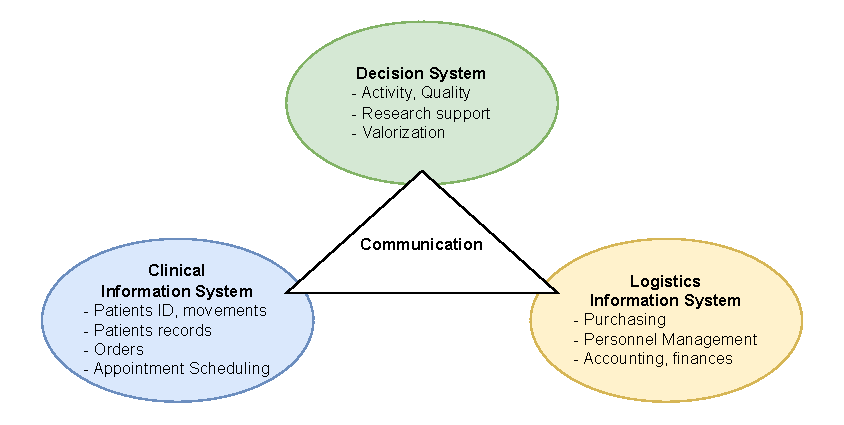
\includegraphics[width=0.9\textwidth]{figures/HIS Schema.pdf} 
    \caption{Functional subsystems in a Hospital Information System, adapted from~\cite{Degoulet_2014}.}
    \label{fig:his-functional}
\end{figure}

The design of a \ac{HIS} is generally component-based~\cite{Van_De_Velde_Degoulet_2003, Winter_Ammenwerth_Haux_Marschollek_Steiner_Jahn_2023}.
%
The components of a \ac{HIS} follow a functional decomposition~\cite{Winter_Ammenwerth_Haux_Marschollek_Steiner_Jahn_2023} separating the core functionalities across different processes. 
%
Classical components of a \ac{HIS} include~\cite{Winter_Ammenwerth_Haux_Marschollek_Steiner_Jahn_2023}:
\begin{itemize}
    \item Patient Administration Systems including \textbf{Patient Identification}, \textbf{Appointment Scheduling (AS)}, \textbf{Admission, Discharge and Transfer (ADT)} and \textbf{Billing and Accounting};
    \item Medical Documentation Systems such as the \textbf{\acp{EHR}} to manage patient medical records, including clinical notes, diagnoses, medications, and allergies, now often integrated to provide a full view of patient data through \textbf{Clinical Data Repositories (CDR)};
    \item \textbf{Operation Management Systems} to support logistics such as planning, bed management and staff schedules for surgeries.
    \item \textbf{Computerized Physician Order Entry (CPOE)} to manage orders for medications, lab tests, imaging, and other procedures;
    \item \textbf{Clinical Decision Support Systems (CDSS)} to provide clinicians with evidence-based recommendations and alerts to support clinical decisions;
    \item ancillary departmental systems such as \textbf{Laboratory Information Systems (LIS)} to manage laboratory tests and results, \textbf{Radiology Information Systems (RIS)} and \textbf{Picture Archiving and Communication Systems (PACS)} to manage imaging studies and results, and \textbf{Pharmacy Information Systems (PIS)} to manage medication orders and dispensing;
    \item \textbf{Document Archiving Systems} to store and manage medical documents for archival and legal purposes. 
\end{itemize}

These core modules are often building the backbone of a \ac{HIS} which can then be correlated with a variety of specific additional systems to support specific needs of the organization. 
%
These include telemedicine systems, patient portals, mobile health applications, and systems for managing specific clinical areas such as oncology or cardiology~\cite{Winter_Ammenwerth_Haux_Marschollek_Steiner_Jahn_2023}.

The level of digitalization and integration of these functional components can significantly impact operations in a healthcare organization. 
%
Maturity assessments of \ac{HIS} are hence crucial to identify gaps and areas of improvement.
%
Several maturity models have been proposed~\cite{Gomes_Romão_2018}, assessing the maturity of \ac{HIS} across various dimensions such as technology, processes, and organizational culture.

A notable example is the \emph{Electronic Medical Record Adoption Model (EMRAM)} by HIMSS~\cite{HIMSS_EMRAM_Criteria}, which assesses the adoption and utilization of electronic medical records in healthcare organizations across eight stages, from 0 (no electronic records) to 7 (fully electronic and integrated systems).
%
The different levels offer a roadmap for healthcare organization to plan their digital transformation journey. 
%
Interestingly, the first levels (following also an historical perspective) focus on the digitalization of ancillary systems first, and follow with the integration of \ac{EHR} in clinical data repositories, highlighting the importance of data integration as a key step in the digital transformation of healthcare organizations.

Other models such as the one proposed in \cite{Carvalho_Rocha_van_de_Wetering_Abreu_2019} also identify different levels, characterizing the maturity of \ac{HIS} in terms of interoperability, data analysis, strategic planning, involved people, availability of electronic medical records, security and technological infrastructure. 
%
The goal of the last levels is to achieve a fully national integrated \ac{HIS} that utilizes real-time data, supports personalized medicine, flexible planning and clinical decision-making, in line with the goals of Healthcare 4.0.

%=======================================================
\section{Medical Standards for Interoperability}
%=======================================================

The complexity of \acp{HIS} and the need for integration across different systems make interoperability a key requirement. 
%
This motivates the need for standards to ensure that different systems can communicate and exchange data effectively. 
%
The complexity of medical data and the variability in medical processes makes the encoding of medical knowledge in such standards a challenging task. 

Over the years, several independent organizations have developed standards to address different aspects of healthcare interoperability~\cite{benson2016principles}.
%
Medical interoperability standards can be broadly categorized into different types based on their purpose and scope: 
\begin{itemize}
    \item \textbf{Terminologies and Coding Systems} provide a common vocabulary for representing medical concepts, diagnoses, procedures and medications. Examples include \ac{ICD} (established by the World Health Organization) for disease classification, \ac{SNOMED-CT} for clinical terminology, and \ac{LOINC} for laboratory and clinical observations.
    \item \textbf{Data Exchange and Transport} standards define how data is exchanged between systems. One of the main example is \ac{HL7} Clinical data Architecture and its new version \ac{FHIR}, which defines a structured information model for exchange of medical data across systems.
    \item \textbf{Specialized Document Formats} are used to represent specific types of medical documents. An example is the \ac{DICOM} standard for medical imaging.
\end{itemize}

These standards are often used in combination to achieve technical and semantic interoperability. 
%
In particular, \ac{FHIR} is the most modern proposal for data exchange in healthcare systems, adopting a modular approach based on the definition of \emph{resources} that can be combined to represent complex clinical concepts, which can be associated with other standard terminologies~\cite{Braunstein_2018}
%
\ac{FHIR} adopts a \ac{REST}~\cite{fielding2000architectural} approach to its \ac{API}, making it easier to integrate with modern Web technologies, breaking out of the traditional silos of healthcare systems. 
%
Despite this choice, \ac{FHIR} is not limited to work in a request-response fashion, but can be integrated as a transport protocol for other communication paradigms such as publish-subscribe or event-based architectures, or even simply to serialize documents for archival purposes~\cite{benson2016principles}.
%
\ac{FHIR} resources can link to other resources, enabling the representation of relationships between entities (e.g., patients, practitioners, medications, observations). 
%
This approach favors the integration of data from multiple sources in a \ac{HIS}, and the pervasive use of \ac{FHIR} as a the format to represent and exchange data in a structured format~\cite{benson2016principles}.

\todo{an image for FHIR?}

\ac{FHIR} resources have a hierarchical structure, with each resource having a defined set of attributes and relationships to other resources.
%
The semantic interpretation of \ac{FHIR} resources is supported by a fixed set of data types, and the support for referencing external terminologies and coding systems, providing unambiguous meaning to the data being exchanged.
%
Furthermore, \ac{FHIR} provides a mechanism for defining profiles and extensions, allowing customization of resources to meet specific use cases while maintaining interoperability with the core standard. 

Due to its versatility and modern design, \ac{FHIR} is increasingly being adopted in healthcare systems~\cite{Ayaz_Pasha_Alzahrani_Budiarto_Stiawan_2021} and also in healthcare research~\cite{Vorisek_Lehne_Klopfenstein_Mayer_Bartschke_Haese_Thun_2022}, making it a key standard for healthcare interoperability today.

A different approach to \ac{EHR} interoperability is taken by the openEHR standards~\cite{openEHR_architecture_overview}, which focus on the multi-level definition of stable \emph{reference models} and domain-specific \emph{archetypes} to represent clinical concepts in a structured and reusable way.
%
The main focus of openEHR is on the modeling of clinical data, rather than on the exchange of data between systems.
%
This makes openEHR more suitable for the design of clinical data repositories and \ac{EHR} systems~\cite{Delussu_Frexia_Mascia_Sulis_Meloni_Del_Rio_Lianas_2024}.
%
The standard further provides guidelines on management of \ac{EHR} including versioning, auditing and access control which are crucial for the management of sensitive medical data. 
%
OpenEHR can hence be considered complementary to other standards, focusing on the management and storage of \ac{EHR} data~\cite{Bosca_Moner_Maldonado_Robles_2015,Pedrera-Jiménez_García-Barrio_Frid_Moner_Boscá-Tomás_Lozano-Rubí_Kalra_Beale_Muñoz-Carrero_Serrano-Balazote_2023}. 

This section provides a brief overview of the main standards for healthcare interoperability. 
%
The abundance of standards clearly reflects the complexity of the healthcare domain both in terms of the intrinsic complexity of medical data and processes and the variety of stakeholders and organizations involved.
%
Adopting and combining effectively these standards is a key requirement for the design of modern \acp{HIS} towards the implementation of Healthcare 4.0 objectives.
%
Semantic interoperability is still an open challenge as the standards partially overlap and are not supported by formal ontological models which could remove ambiguities and improve deductive reasoning~\cite{de_Mello_Rigo_da_Costa_da_Rosa_Righi_Donida_Bez_Schunke_2022}.
%
In this sense, alignment with Semantic Web technologies~\cite{berners2023semantic} and ontologies could provide a pathway towards achieving greater semantic interoperability in healthcare~\cite{Schulz_Martínez-Costa_2013}.

%=======================================================
\section{Intelligent Applications in Healthcare}
%=======================================================

\todo{maybe find an image for AI applications..}

Among the drivers of Healthcare 4.0, \ac{AI} is playing an increasingly important role in healthcare.
%
Due to its inherent complexity, healthcare has always been a target domain for \ac{AI} applications, as the possibility to ease the burden of healthcare professionals and improve the quality of care is a strong motivation for innovation. 
%
While originally most \ac{AI} applications in healthcare focused on rule-based symbolic reasoning and expert decision-support systems to support clinical decisions, the recent advantages in \ac{ML} and \ac{DL} and the availability of large amounts of data have made data-driven approaches more feasible~\cite{Yu_Beam_Kohane_2018}.
%
Recent surveys confirm that the rate of scientific publications on \ac{AI} in healthcare is growing at a very fast pace covering a wide range of applications~\cite{Secinaro_Calandra_Secinaro_Muthurangu_Biancone_2021,Yousefi_Dehnavieh_Laberge_Gagnon_Ghaemi_Nadali_Azizi_2025}.

Applications of \ac{AI} techniques in healthcare span across a wide range of areas.
%
One of the most significant is image-based diagnosis, where \acp{CNN} for image classification have shown performances comparable or even superior to human experts in recognizing pathologies from medical images.
%
Other relevant applications include genome interpretation, biomarker discovery, risk estimation and prediction of clinical outcomes, and continuous monitoring through \ac{IoT} stream analysis~\cite{Yu_Beam_Kohane_2018}.

More recently, the advent of \acp{LLM} and \ac{GenAI} technologies is opening new possibilities for \ac{AI} applications in healthcare~\cite{Sai_Gaur_Sai_Chamola_Guizani_Rodrigues_2024}.
%
\ac{GenAI} techniques can be used for data augmentation, to generate synthetic medical data and support training of \ac{ML} models when real data is scarce. 
%
\acp{LLM} can be used to analyze and produce medical documents and their adoption is growing at a fast pace especially for the automatic draft of clinical documentation from conversations with the overall objective of increasing efficiency by automating repetitive tasks~\cite{Poon_Lemak_Rojas_Guptill_Classen_2025}.
%
Additionally, \ac{LLM} can be used to interact with patients through chatbots, providing information and support for common medical questions and concerns.
%
Fine-tuned medical \acp{LLM} can also be used to support clinical decision-making and summarization of medical literature~\cite{Sai_Gaur_Sai_Chamola_Guizani_Rodrigues_2024}.

Secinaro et al.~\cite{Secinaro_Calandra_Secinaro_Muthurangu_Biancone_2021} identify three main clusters of application of \ac{AI} in healthcare:
\begin{itemize}
    \item predictive models for diagnosis and monitoring of patients
    \item decision support systems to support decision-making
    \item big data analytics to optimize healthcare operations and management
\end{itemize}

This multi-faceted approach highlights the wide scope of \ac{AI} applications in healthcare which can target both clinical and administrative processes.

Given the critical nature of healthcare, the adoption of \ac{AI} requires careful consideration of ethical implications~\cite{Morley_Machado_Burr_Cowls_Joshi_Taddeo_Floridi_2020}.
%
In general \ac{AI} systems are seen as tools to improve human decision-making, making it possibly more objective and data driven.
%
Of course this requires carefully designed systems and data collection processes to avoid introducing new sources of errors and biases which may undermine the benefits~\cite{Norori_Hu_Aellen_Faraci_Tzovara_2021}.

The reliance on \ac{AI} systems for clinical decisions can also raise concerns of misdiagnosis due to the possibility of overestimating the confidence of automated systems~\cite{Morley_Machado_Burr_Cowls_Joshi_Taddeo_Floridi_2020}.
%
New trends are hence focusing on explainability and interpretability of \ac{AI} systems which becomes a crucial property for the deployment of \ac{AI} systems in healthcare~\cite{Bharati_Mondal_Podder_2024}.
%
\ac{XAI} techniques are being increasingly required in healthcare~\cite{Freyer_Groß_Lipprandt_2024} settings due to the need for transparency in the decision-making process which is crucial for building trust: a necessary condition for the successful acceptance of \ac{AI} by both patients and healthcare professionals~\cite{Alonso_Astobiza_Ortega_Lozano_2025}.

Finally, regulations play a crucial role in the effort to ensure that \ac{AI} systems in healthcare are safe and ethical~\cite{Freyer_Groß_Lipprandt_2024}.
%
These need to be accompanied by guidelines and best practices that promote careful design and implementation of \ac{AI} models, from data collection, selection and preprocessing, to model training and validation~\cite{de_Hond_Leeuwenberg_Hooft_Kant_Nijman_van_Os_Aardoom_Debray_Schuit_van_Smeden_et_al._2022}.


%=======================================================
\section{The \ausl{} Context}
%=======================================================

\auslLong{} is the local public healthcare administration for the Emilia-Romagna region in Italy, covering a population of more than 1.1 million people across a territory of roughly 5100 km$^2$ which covers the provinces of Ravenna, Forlì-Cesena and Rimini and is divided into 8 health districts (\Cref{fig:ausl-map}).
%
The organization manages 7 main hospitals hubs comprising a total of 13 hospital facilities and several other care centers managed by a network of more than 16 thousands employees. 
%
Born from the merger of three different local healthcare administrations in 2013, \ausl{} is among the largest healthcare providers in Italy.
%
The high complexity of the organization and the large territory it covers make \ausl{} a relevant case study for the challenges of digital transformation in healthcare as, due to its historical evolution it deals with integration of heterogeneous systems and processes across different settings and can represent a microcosm of the challenges faced by the healthcare sector in general.


\begin{figure}[t]
    \centering
    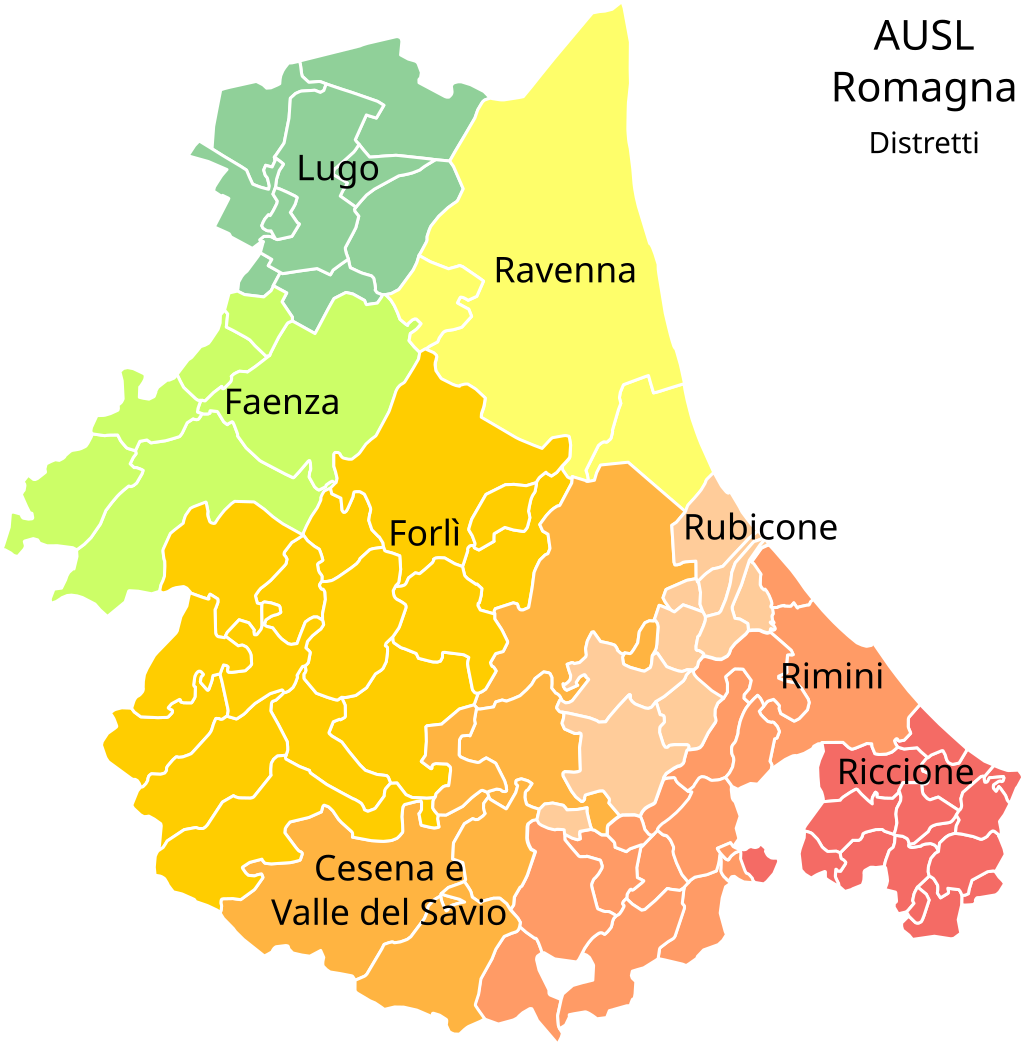
\includegraphics[width=0.55\textwidth]{figures/mappa_ausl.png} 
    \caption{
        Map of the \ausl{} territory, credits:
        \url{https://commons.wikimedia.org/wiki/File:Mappa_dell\%27AUSL_Romagna.svg}
    }
    \label{fig:ausl-map}
\end{figure}


\ausl{}, aligned with the objectives of the national healthcare plans, is pursuing a digital transformation process aimed at improving the efficiency and effectiveness of its services.
%
A first essential step in this direction has been the adoption of a personal \ac{EHR} system directly accessible by patients (\emph{Fascicolo Sanitario Elettronico (FSE)}).
This system allows patients to access their health records, book appointments, and communicate with healthcare providers more easily. 
%
Emilia-Romagna has been the Italian region with the highest success rate in the implementation of FSE~\cite{fse_ausl_prima} with over 65\% of the population having accessed their FSE at least once and more than 90\% of the population agreeing to its consultation by healthcare professionals.

The digitalization program has been accelerated by the COVID-19 pandemic, which has highlighted the need for more agile and resilient healthcare systems worldwide.
%
The NextGenerationEU programme of the European Union funds several initiatives in its member states as a response to the COVID-19 pandemic. 
%
In Italy, this has been translated into the \emph{Piano Nazionale di Ripresa e Resilienza (PNRR)} which includes several \emph{missions}.
Mission 1 includes as a key objective the which digitalization of public administrations, including healthcare organizations. 
Mission 6 is instead entirely dedicated to the innovation of healthcare services, targeting the technological improvement of hospitals, decentralization of healthcare services, telemedicine and remote care~\cite{italy_pnrr_2021}.
%
This PhD work is also funded under PNRR, under Mission 4 promoting the collaboration of industrial partners and research institutions.

\ausl{} is continuing its digital transformation journey within this framework.
%
A strategic plan for its digitalization (``Progetto Sanità Digitale'') has been defined in 2021 to guide the process as a collaboration between \ausl{}, the Computer Science and Engineering Department of the University of Bologna and the oncologic care and research center {Istituto Romagnolo per lo Studio dei Tumori ``Dino Amadori''(IRST)}, members of a local lavoratory for healthcare innovation (Laboratiorio Sanità Digitale~\footnote{\url{https://laboratorio-sanita-digitale.github.io/}})~\cite{progetto_sanità_digitale}.
%
Key objectives of the digitalization plan include the decentralization and distribution of care with local care centers and remote monitoring, the integration of data from multiple sources to support personalized medicine and the improvement of operational efficiency. 
%
A strategic technology envisioned in this context is the adoption of \emph{\acp{DT}~\cite{Grieves_2023}}, which can offer an aggregation point for data and functionalities from multiple systems tailored to the representation of critical assets in the healthcare organization~\cite{progetto_sanità_digitale}.

This thesis work is framed within this context, exploring the role of \acp{DT} as enablers of Healthcare 4.0 objectives and focusing on the challenges of interoperability and data integration in a complex and distributed healthcare organization such as \ausl{}.

%=======================================================
\section{Final Remarks}
%=======================================================

This chapter provides an overview of the context of Healthcare 4.0 which motivates and frames the work presented in this thesis. 
%
The digital transformation of healthcare is a complex process that involve multiple dimensions, from technological to organizational and socio-economic factors.

The chapter highlights the multi-faceted nature of the healthcare domain, and the efforts that are being pursued towards improving digitalization, with a focus on \ac{HIS} as the exemplary case of \ac{ICT} systems in healthcare which motivates the need for interoperability and data integration.

The chapter further reflects on the role of \ac{AI} in healthcare, showing how it can address both clinical and organizational challenges, emphasizing the critical requirements the domain imposes on the design of intelligent applications that are trustworthy, reliable and fair.

Finally, the chapter describes the context of \ausl{} as the partner organization for this thesis work, highlighting the relevance of the challenges faced by the organization in its digital transformation journey which motivate this thesis work. 